\phantomsection
%\addcontentsline{toc}{chapter}{Introduzione}
\chapter{Introduzione}
\markboth{Introduzione}{}
% [titolo ridotto se non ci dovesse stare] {titolo completo}

\section{Contesto applicativo} 
Con l'espansione e la crescita della digitalizzazione in tutti gli ambiti della nostra società, si è verificato un aumento significativo di fenomeni criminali in ambito digitale, la sicurezza informatica nasce con il proposito di contrastare e annullare questa tipologia di criminalità.
La sicurezza informatica non ha come scopo solo quello di evitare attacchi informatici ma anche quello di offrire software o dispositivi capaci di essere robusti e affidabili, evitando che questi possano essere compromessi.
\newline La crescita dello spazio cibernetico ovvero l'interconnessione delle infrastrutture informatiche \citep{dei2013quadro} ha reso i sistemi informatici su cui si fonda più vulnerabili a possibili manipolazioni, con l'avanzare degli anni tutto ciò sta causando una crescita graduale degli attacchi informatici nel mondo, i quali stanno diventano sempre più frequenti e complessi coinvolgendo sempre più tipologie di vittime e causando danni economici sempre maggiori.
Lo sviluppo della criminalità informatica è dovuto anche al modo in cui possono operare gli hacker, infatti lo spazio cibernetico consente loro di poter compiere un attacco i qualsiasi posizione fisica colpendo in modo istantaneo l'obiettivo e in modo quasi del tutto anonimo. \newline 
Internet è nato come un' \textit{ungoverned space} ovvero non regolamentato da autorità politiche o internazionali \citep{baldoni2015futuro}, tuttavia a causa di una maggiore pressione in ambito di sicurezza pubblica e a causa di attacchi che in più situazioni hanno coinvolto enti nazionali, diverse nazioni si stanno mobilitando per cercare di offrire più sicurezza online ai propri cittadini.
\begin{figure}[!htb]
    \centering
    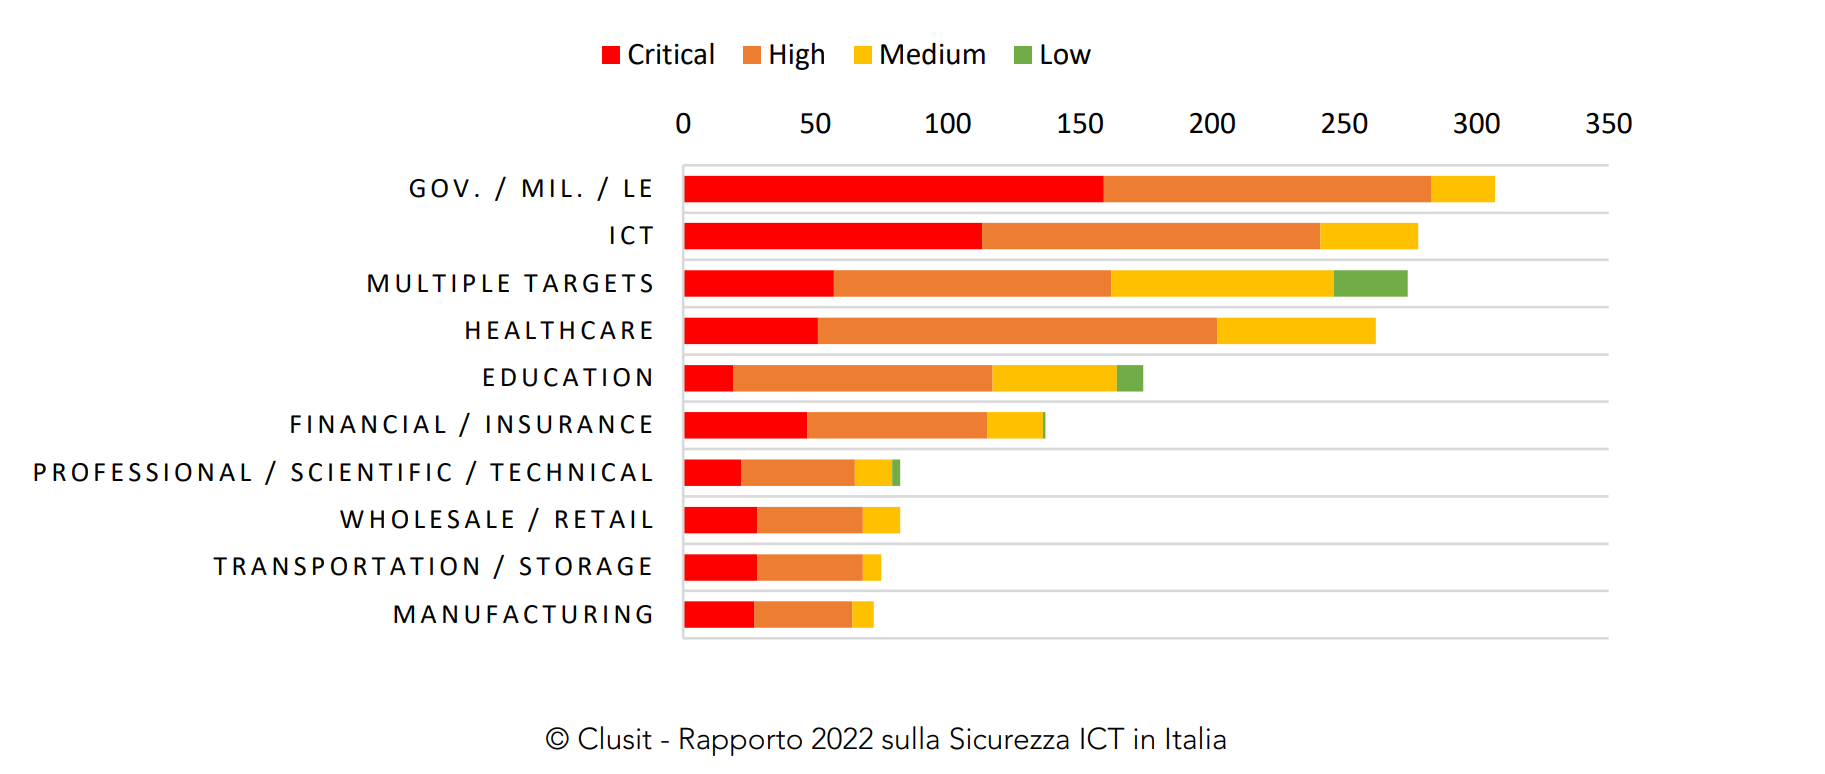
\includegraphics[scale=0.7]{../figure/target.png}
    \caption{Top 10 vittime 2021 in Italia}
    \label{fig:top10vittime}
\end{figure}
In questo senso uno degli attacchi hacker che ha fatto molto discutere in Italia è avvenuto il 30 luglio 2021 al CED (centro elaborazione dati) della regione Lazio \citep{LazioAttack}, l'attacco ha mandato in tilt i servizi di privati e aziende, coinvolgendo anche il sistema sanitario della regione dedicato alla vaccinazione contro il COVID-19, gli effetti sono stati molto gravi provocando un mese di interruzione di alcuni servizi tra cui alcuni urbanistici, ma coinvolgendo sopratutto servizi sanitari online. L'attacco informatico subito è definito \textit{ransomware} \citep{Ransomware} questa tipologia di attacco si diffonde attraverso un programma dannoso (malware), che ha come scopo quello di bloccare l'accesso ai contenuti presenti sul dispositivo infetto, per poi richiedere un riscatto per renderli di nuovo accessibili, nel caso della regione Lazio dalle ricostruzioni l'infezione è partita da un computer di un dipendente, dal quale i criminali sono riusciti ad accedere ai servizi di un dipendente con privilegi di admin, tramite quest'ultimo sono riusciti ad accedere ai dati per poi criptarli. 
\newline Attacchi come quello avvenuto alla regione Lazio mostrano come queste attività criminali possono incidere notevolmente sulla sicurezza delle istituzioni e dei cittadini, questi eventi stanno portando gli enti nazionali e internazionali a mobilitarsi per poter prevenire e combattere questa tipologia di criminalità.
\begin{figure}[!htb]
    \centering
    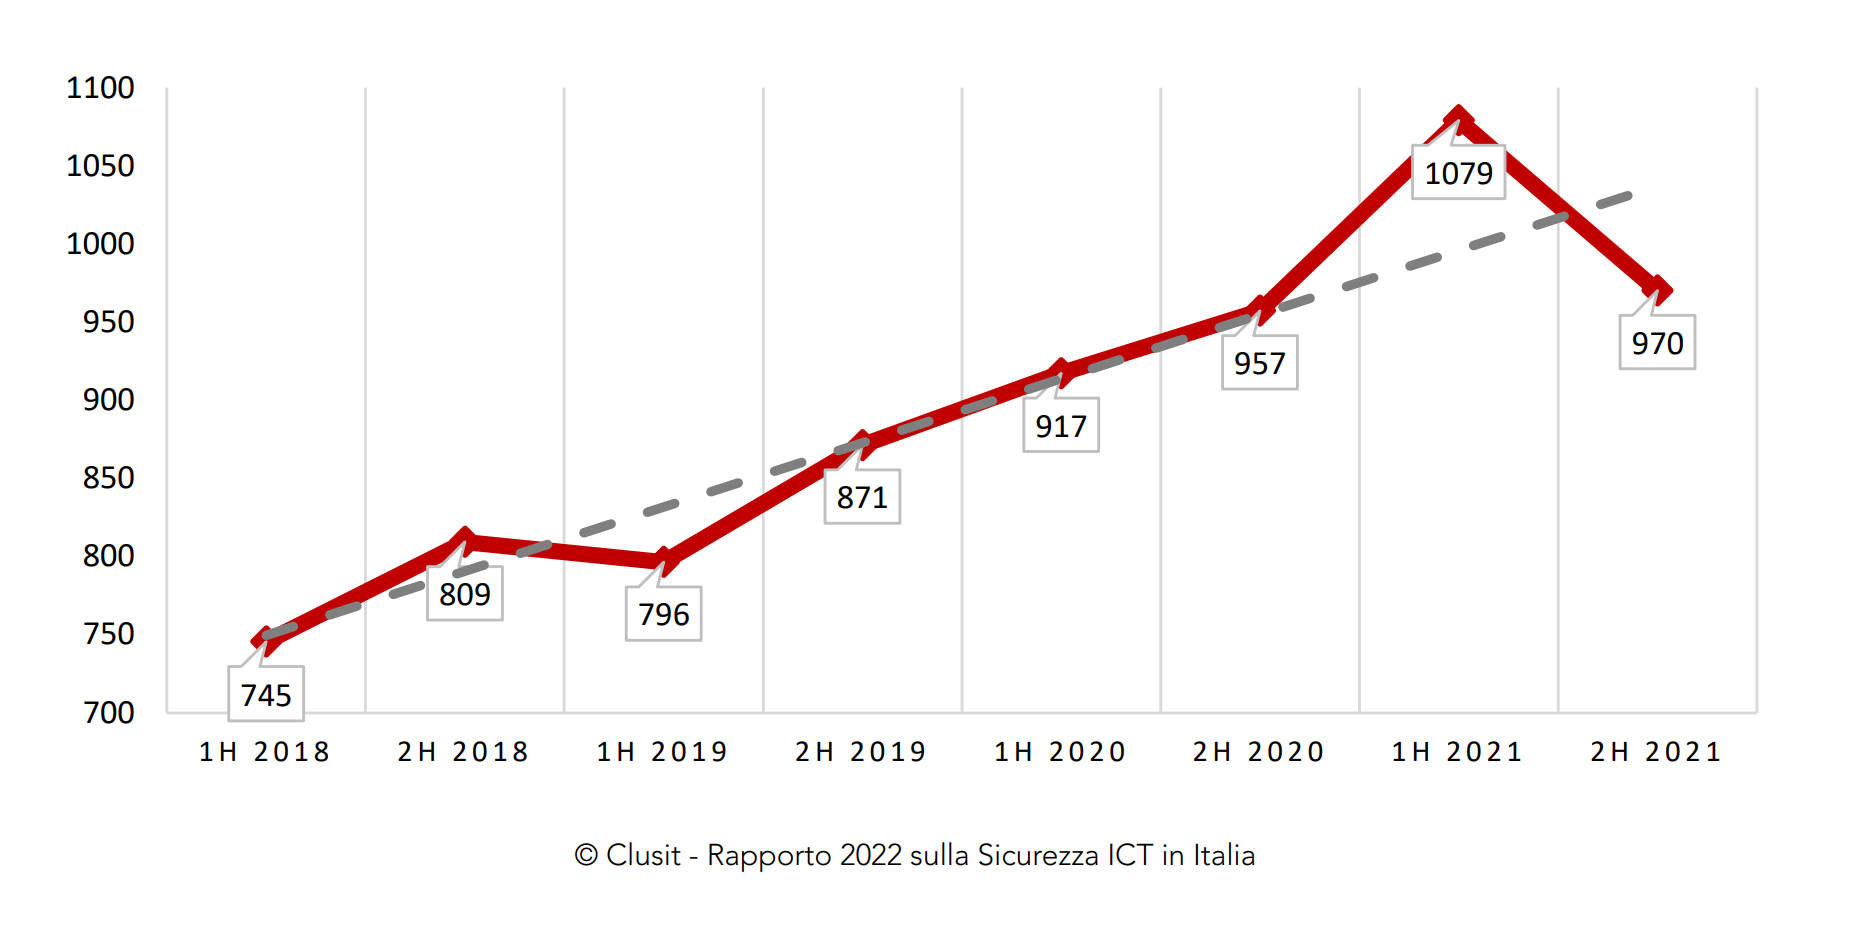
\includegraphics[scale=0.8]{../figure/attacchi per semestre.png}
    \caption{Attacchi per semestre dal 2018}
    \label{fig:attacchiPerSemetre}
\end{figure}
\newline In Italia, negli ultimi anni, il tema della sicurezza informatica sta assumendo una posizione sempre più rilevante, uno degli interventi più importanti è il decreto-legge n. 105 del 2019 il quale è nato con lo scopo di garantire un elevato livello di sicurezza delle reti e dei sistemi informatici delle pubbliche amministrazioni, dei servizi informatici e degli enti e operatori nazionali \cite{SicurezzaCibernetica}. Attualmente la sicurezza cibernetica è uno dei progetti principali finanziati dal \textit{PNRR} (Piano nazionale di ripresa e resilienza) \citep{italiano2021piano}, a cui sono destinati 620 milioni di euro per il rafforzamento delle infrastrutture legate alla protezione cibernetica in Italia. 
Anche l'Europa attraverso la Commissione europea sta spingendo gli Stati membri a rafforzare le proprie difese informatiche, in particolare nel 2016 è stata introdotta la prima misura legislativa per tutta l'Europa in ambito di sicurezza cibernetica, la \textit{Direttiva NIS} \citep{nis}, che poi, a fronte di una notevole accelerazione della digitalizzazione causata dalla crisi COVID-19, la Commissione europea nel dicembre del 2020 ha proposto la direttiva NIS riveduta (\textit{NIS2})\citep{nis2}.
\newline Con il trascorrere degli anni il numero degli attacchi informatici sta aumentando, con essa sta crescendo la gravità degli attacchi e la loro complessità, aumentando i costi ad esso associati. Il \textbf{Clusit} (Associazione Italiana per la Sicurezza Informatica) \citep{clusit} periodicamente rilascia report sulla situazione italiana in ambito di sicurezza informatica, nell'ultimo rapporto avvenuto a marzo del 2022 \citep{clusitReport} il Clusit ha riportato che nel 2021 il numero di attacchi informatici nel mondo ha registrato un aumento di circa 10\% rispetto al 2020, un dato molto preoccupante è l'aumento dell'impatto degli attacchi infatti il 79\% di questi ha avuto un impatto elevato. Un importante analisi è stata condotta per il territorio italiano che ci permette di analizzare la situazione in Italia, dalla figura~\ref{fig:attacchiPerSemetre} possiamo denotare come dal 2018 il numero di attacchi in Italia è cresciuto enormemente, con un picco di 1079 attacchi nel primo semestre del 2021, un dato molto importante da considerare in ambito di sicurezza informatica sono le vittime degli attacchi, infatti gran parte di queste, come si evince dalla figura \ref{fig:top10vittime}, sono enti nazionali e governativi, rispetto al 2020 però le categorie che hanno avuto un aumento considerevole di attacchi nell'ultimo anno sono Transportation/Storage con un aumento del 93,3\% e la categoria di News/Multimedia con un aumento del 60,5\%. \newline
\begin{figure}
    \centering
    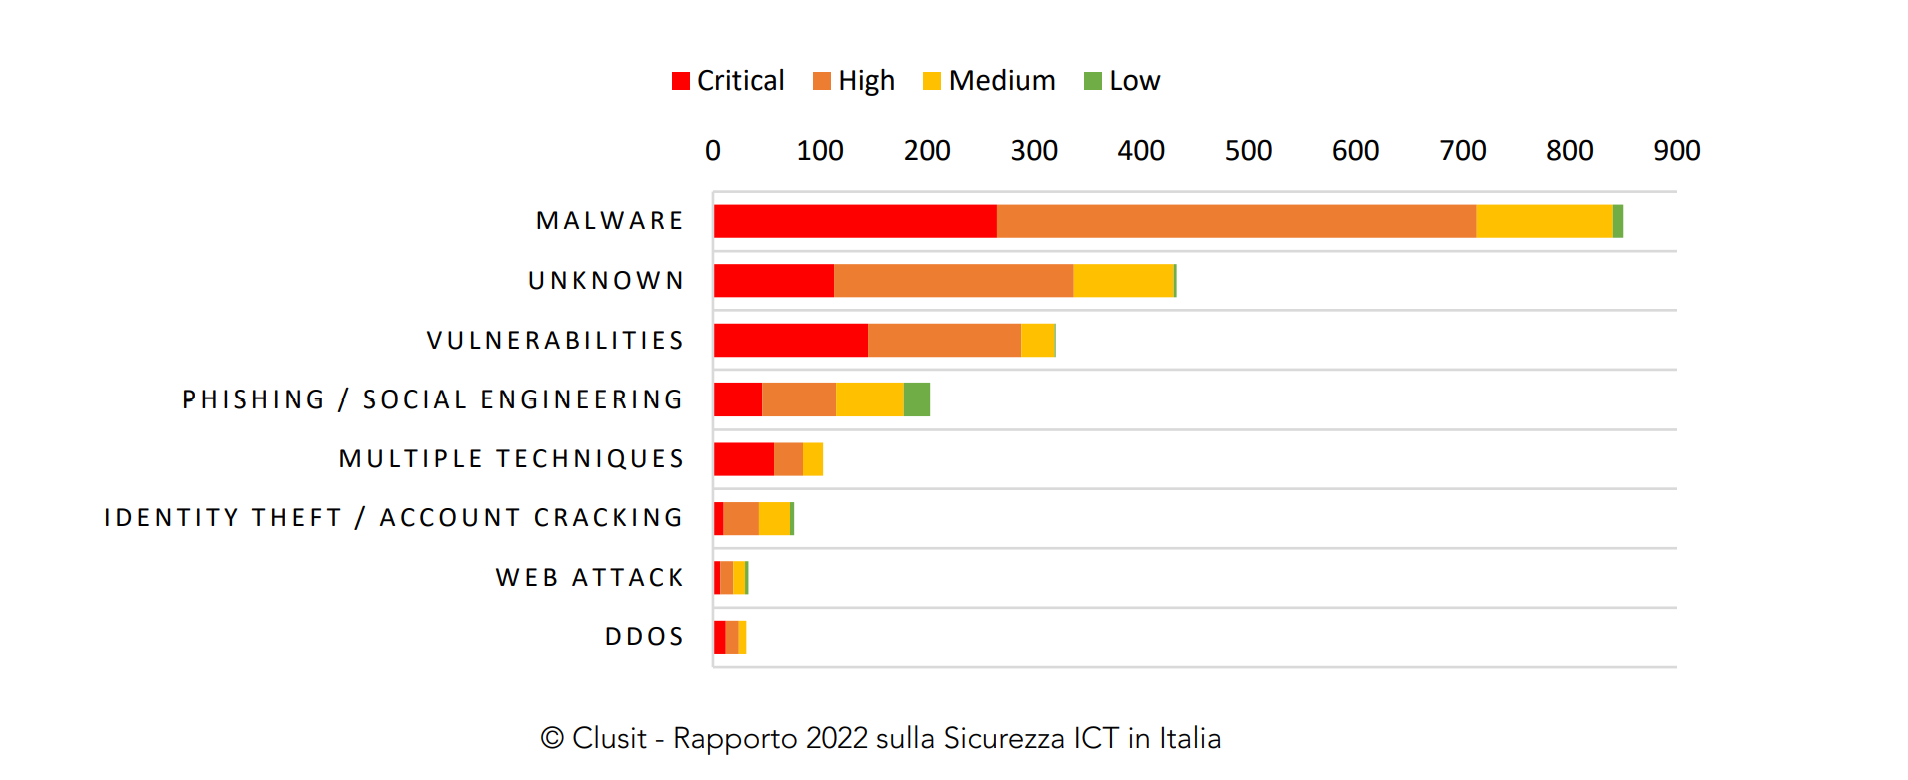
\includegraphics[scale=0.8]{../figure/clusit attacchi.png}
    \caption{Tecniche di attacco 2021}
    \label{fig:tecnicheDiAttacco}
\end{figure}
\begin{figure}
    \centering
    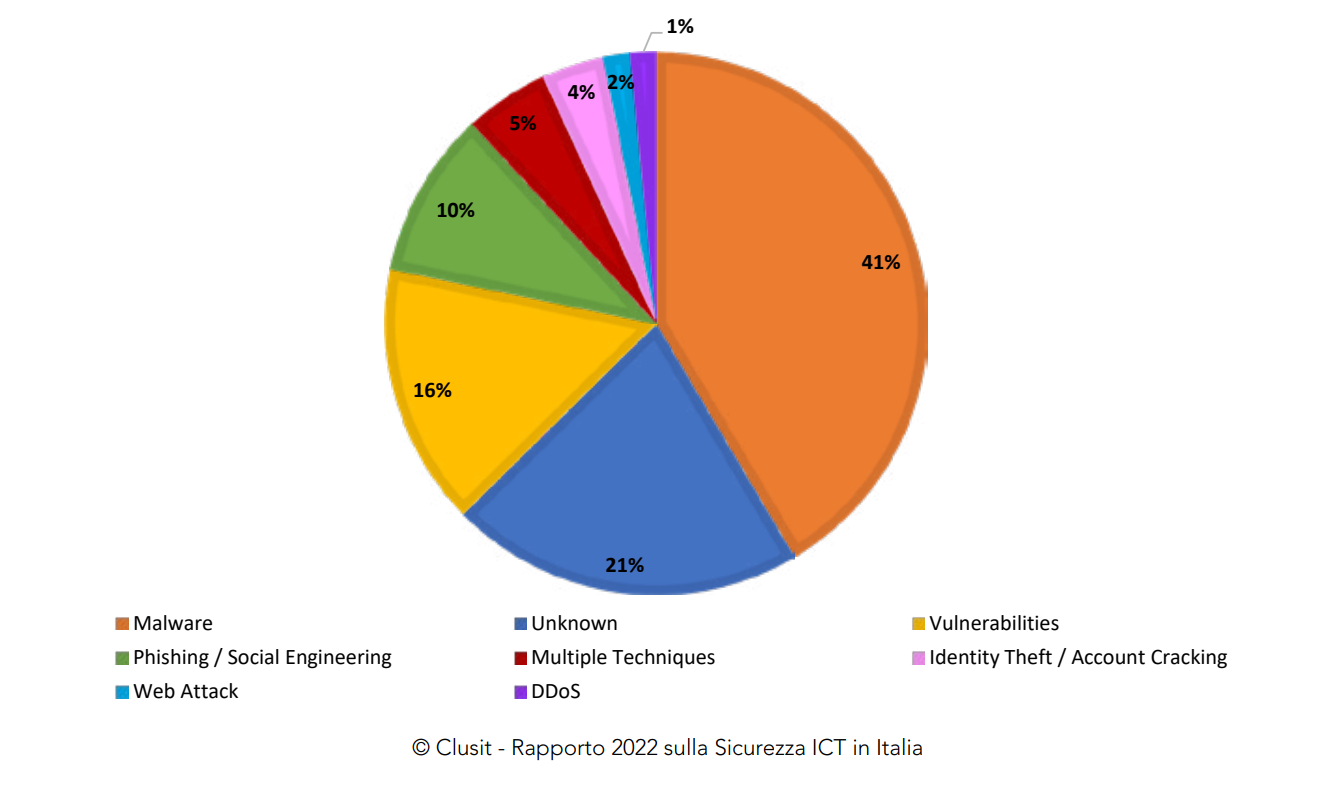
\includegraphics[scale=0.9]{../figure/tipologiaAttacchiTorta.png}
    \caption{Distribuzione tecniche di attacco 2021}
    \label{fig:tecnicheDiAttaccoTorta}
\end{figure}
Uno dei dati più interessanti anche in termini di prevenzione è il modo attraverso cui gli hacker riescono ad effettuare un attacco informatico, figura \ref{fig:tecnicheDiAttacco} e figura \ref{fig:tecnicheDiAttaccoTorta} ci mostrano quali sono e in che modo sono distribuiti, da quanto possiamo notare il metodo più diffuso sono i malware con una percentuale del 41\%, mentre il 21\% è sconosciuto e il 16\% degli attacchi avviene sfruttando vulnerabilità, inoltre confrontando i dati con l'anno precedente notiamo un notevole aumento di attacchi avvenuti sfruttando vulnerabilità con un aumento del 60\% di quest'ultimi, mentre i malware hanno registrato un aumento del 9.7\%, oltre a questi dati notiamo anche un incremento dell'impatto di quest'ultimi, anche in questo caso le vulnerabilità hanno registrato un aumento soprattutto di attacchi critici e alti.
\newline Come mostrato gli aspetti più critici della sicurezza informatica sono lato software, per questo motivo gran parte degli studi coinvolti in ambito di sicurezza si concentrano sui sistemi software.
La sicurezza di un sistema software nasce dalla sua origine, durante la definizione dei requisiti, in particolare durante questa fase sono definite le politiche di sicurezza che specificano ciò che è consentito e ciò che non è consentito dal sistema, più nel dettaglio definiscono la disponibilità del sistema e la definizione per ogni tipologia di utente di cosa può fare e a cosa può accedere e nel caso questi requisiti non vengano rispettati come il sistema deve comportarsi, in modo tale funzionare correttamente in caso di un errore o in caso di un attacco al sistema \citep{bishop2003computer}.
Questo mostra come un buon sviluppo del software può in parte contribuire con la creazione di un prodotto software sicuro da possibili attacchi informatici, sfortunatamente, tutto ciò non è sufficiente per evitare la presenza di possibili vulnerabilità software.

\section{Motivazioni e Obiettivi} %\label{1sec:scopo}
Come abbiamo visto la sicurezza informatica è uno dei problemi più rilevanti in campo informatico, che colpisce principalmente persone e istituzioni, attaccando la loro sicurezza e minando profondamente la salute e la privacy degli utenti. Quindi combattere la diffusione di attacchi informatici non solo ci permette di contrastare organizzazioni criminali e truffe, ma anche a salvaguardare la sicurezza nazionale, internazionale e dei singoli cittadini, la lotta contro la criminalità informatica ci permette inoltre di abbassare drasticamente i costi dovuti a danni o a truffe online.
\newline La prevenzione è uno dei metodi più efficaci per abbattere l'aumento di crimini informatici, un'infrastruttura o un prodotto software che offrono buoni sistemi di protezione contro possibili attacchi informatici sono meno vulnerabili e più affidabili, quindi sono più difficili da compromettere, lato software la realizzazione di sistemi sicuri, prevede inevitabilmente un innalzo dei costi di implementazione, sfortunatamente a causa di budget ridotti solitamente per sistemi software medio-piccoli si tende a raggiungere un compromesso tra budget (in termini di denaro e tempi di sviluppo) con requisiti del prodotto tra cui il grado di sicurezza di questo, tutto ciò però inevitabilmente crea un deficit di sicurezza in che rende il sistema software non del tutto sicuro e affidabile.
\newline Il mio lavoro di tesi si pone l'obiettivo di trattare e analizzare la terza categoria di attacchi informatici più diffusi in Italia, ovvero le vulnerabilità, nello specifico il mio studio si concentrerà sulle tecniche di individuazione delle vulnerabilità software attraverso modelli di predizione basati su machine learning. L'obiettivo è minimizzare l'introduzione di vulnerabilità in un progetto software e di minimizzare i costi ad esso associati, favorendo anche l'individuazione di vulnerabilità in fase di implementazione, testing e manutenzione di un progetto software, rendendo quest'ultimo più sicuro e affidabile.

\section{Risultati ottenuti}
Nella prima parte di questo studio la mia attenzione è stata posta sullo studio e l'analisi delle vulnerabilità software, come queste possono essere introdotte all'interno di un prodotto software, in che modo possono essere usate dai criminali informatici e che impatto possono avere sulle aziende produttrici e sui loro clienti, in questa prima fase ho analizzato diversi studi fatti in questo ambito, particolare attenzione in questa fase è stata rivolta sui VPM (modelli di predizione di vulnerabilità) e sulle performance ottenute da quest'ultimi in vari ambiti. A seguito di quanto appreso da lavori antecedenti, ho compreso come e in che modo costruire il modello di predizione definendo obiettivi, ambito applicativo e le fasi di implementazione del modello. \newline Il contesto applicativo scelto sono applicazioni Java e il modello di machine learning ha come obiettivo la predizione di vulnerabilità a livello di singoli file, questo studio ha come ulteriore scopo di indagare sulla correlazione di diverse metriche software con la presenza di vulnerabilità software. Successivamente sono passato alla parte implementativa, in una prima fase la mia attenzione è stata rivolta sui dati e sul dataset di partenza per il modello di machine learning, ho deciso di creare due dataset distinti a partire da due progetti open source di diversa complessità e grandezza, successivamente ho creato il modello di machine learning attraverso l'uso della libreria Python Scikit learn.
L'implementazione è avvenuta analizzando e implementando diverse tipologie di classificatori, in modo tale da analizzare le differenze in termini di prestazioni e risultati in questo ambito utilizzando diversi classificatori.
Analizzando i risultati ottenuti ho notato una buona accuratezza in quasi tutti i modelli con una percentuale che varia tra l'80\% e 90\%, mentre ho riscontrato per tutti i modelli analizzati un livello di recall più alto rispetto alla precision, il classificatori con indici prestazionali più alti sono stati il \textbf{Decision tree} e il \textbf{Random forest} viceversa il classificatore con risultati più bassi è stato \textbf{Naive Bayes}.


\section{Struttura della tesi}
Nel capitolo~\ref{1cap:background} sono presentate e analizzate le vulnerabilità in campo informatico, con una particolare attenzione rivolta alle vulnerabilità software, successivamente nella seconda parte di questo capitolo sono descritti e analizzati diversi studi fatti in passato per la creazione e l'implementazione dei VPM (modelli di predizione di vulnerabilità) e i risultati ottenuti da quest'ultimi, nell'ultima parte di questo capitolo sono presentati e analizzati diversi dataset utilizzati in passato per la creazione dei VPM. \newline
Nella prima fase del capitolo~\ref{1cap:design} è presente la definizione degli obiettivi posti per la realizzazione del modello di predizione e il contesto applicativo dove quest'ultimo dovrà operare, successivamente c'è la descrizione del lavoro di estrazione dei dati e la costruzione del dataset, e infine il processo di analisi, implementazione e validazione del modello di predizione. \newline
Nel capitolo~\ref{1cap:analisi} sono descritti e analizzati i risultati ottenuti dal modello di machine learning realizzato in questo studio.\newline
Nel capitolo~\ref{1cap:conclusione} sono descritte le conclusioni e possibili sviluppi futuri legati a questo studio.